% !TeX program = tectonic
\documentclass[10pt,a4paper]{article}

\usepackage[margin=2.35cm]{geometry}
\usepackage{amsmath,amssymb,bm}
\usepackage{graphicx}
\usepackage{booktabs}
\usepackage{multirow}
\usepackage{xcolor}
\usepackage{array}
\usepackage[colorlinks=true,linkcolor=blue!60!black,citecolor=green!40!black,urlcolor=blue!60!black]{hyperref}
\usepackage[numbers,sort&compress]{natbib}
\usepackage{caption}
\captionsetup{font=small,labelfont=bf}

\newcommand{\mse}{\mathrm{MSE}}
\newcommand{\cmse}{\mathrm{cMSE}}
\newcommand{\todo}[1]{\textcolor{red}{[TODO: #1]}}
\newcommand{\SpaceTime}{\textsc{SpaceTime}}
\newcommand{\WCM}{\textsc{WCM}}
\newcommand{\optionalfigure}[4]{%
  \IfFileExists{#1}{%
    \begin{figure}[t]
    \centering
    \includegraphics[width=#2\linewidth]{#1}
    \caption{#3}
    \label{#4}
    \end{figure}
  }{}
}

\title{From WCM to SpaceTime: Fixed-Budget Encoding of Longer Visual Histories for Robot Value Prediction}
\author{WCM Project}
\date{September 2026}

\begin{document}
\maketitle

\begin{abstract}
History-aware value models for robot control must use observations collected over time, but simply adding frames increases the visual sequence while leaving the downstream critic with a fixed representational interface. We study a system-level route from an original World Critic Model (WCM) to a \SpaceTime{} history encoder. The central design keeps an eight-frame input and a fixed bottleneck of 64 learned queries while extending the largest sampled temporal offset from $H_{60}$ to $H_{120}$. This isolates temporal span from frame count and latent capacity. On the current two-seed evaluation, both spans improve out-of-distribution (OOD) value-prediction MSE over the original WCM; the $H_{120}$ variant further improves paired OOD MSE over the four-frame input-mosaic reference on the current pair endpoints. The $H_{120}$ experiment is a post-hoc span extension and is therefore reported as a provisional main result pending a third seed and a matched eight-frame mosaic control. We frame the contribution as a fixed-latent-budget history-encoding system, not as a new temporal-attention mechanism or a claim of unrestricted long-horizon compression.
\end{abstract}

\section{Introduction}

Robot value prediction is partially observable: the current image can be compatible with multiple latent states that have different future returns. The original \WCM{} already includes a short local history, but its visual stream does not expose a single, explicit and scalable interface for encoding a long sequence of frames. This creates a practical design question: can a value model use a longer visual history without increasing the number of downstream latent tokens?

We investigate this question through a deliberately narrow route. The model receives eight sparsely sampled frames, applies a shared visual encoder and factorized temporal interaction, and compresses the resulting sequence into $K=64$ learned Perceiver queries. We call the resulting system \SpaceTime{}. We then compare two temporal spans, $H_{60}$ and $H_{120}$, while keeping the frame count, query count, model blocks, initialization protocol, and two-stage training schedule fixed. The experiment is intended to test whether a fixed latent bottleneck can represent a longer history usefully, not whether any temporal-attention primitive is novel.

Our claims are correspondingly bounded:
\begin{enumerate}
  \item We define a concrete \SpaceTime{} encoder for WCM value prediction and make the temporal-span variable explicit.
  \item We evaluate the route from original WCM to fixed-query \SpaceTime{} on common OOD endpoints, using episode-level paired bootstrap intervals and MSE as the primary criterion.
  \item We show a current two-seed result in which extending the span from $H_{60}$ to $H_{120}$ at fixed $K=64$ improves OOD error. The result is provisional until the preplanned third seed and an eight-frame mosaic control are added.
\end{enumerate}

\section{Positioning and scope}

In this paper, ``SpaceTime'' has three layers. It is a method name in the title and abstract, a precisely defined encoder in the method section, and an explanatory space-to-time metaphor in the introduction and discussion. The metaphor does not assert physical spacetime semantics or a causal theorem. Likewise, the paper does not introduce a new temporal-attention family. Its contribution is a system design: a history encoder with a fixed latent bottleneck, evaluated in a value-prediction setting.

The WCM target studied here is the action-free state value $V(s)$. Action enters the separate $Q(s,a)$ head and the action-conditioned dynamics prediction. Those components remain part of the surrounding WCM system but are not presented as new contributions of this paper.

\section{From WCM to SpaceTime}

\subsection{Original WCM}

Let $o_t$ denote the current observation and let $\mathcal{H}_t$ denote the short local history used by the original WCM. The value head predicts
\begin{equation}
  \hat V_t = f_V(\mathcal{H}_t, p_t),
\end{equation}
where $p_t$ denotes proprioceptive features. The value path is action-free. The same WCM system contains an action-conditioned $Q$ path and dynamics path, but neither is needed to define the value target in the experiments below.

\subsection{Temporal sampling and notation}

For a maximum sampled offset $k$, define an eight-frame history
\begin{equation}
  \mathcal{X}^{(k)}_t = \bigl(x_{t-\delta_1},\ldots,x_{t-\delta_8}\bigr), \qquad \max_i \delta_i=k.
\end{equation}
We write $H_k$ for this history. Thus $H_{60}$ and $H_{120}$ both contain eight frames; they differ only in temporal span. In the current experiments,
\begin{align}
  H_{60}:&\quad [0,9,17,26,34,43,51,60],\\
  H_{120}:&\quad [0,17,34,51,69,86,103,120].
\end{align}
The notation does not imply $k$ frames or $k$ seconds.
When an offset crosses an episode boundary, the data loader clamps it to the episode's first frame. Thus increasing $k$ changes the temporal span and the fraction of boundary-clamped histories; it does not guarantee that every sampled frame is an independent observation.

\subsection{Fixed-query history encoder}

Each frame is encoded by a shared visual backbone $\phi$:
\begin{equation}
  z_i = \phi(x_{t-\delta_i}), \qquad i=1,\ldots,8.
\end{equation}
The frame features are processed by factorized temporal interaction layers, followed by a Perceiver-style cross-attention bottleneck with $K$ learned queries $q_1,\ldots,q_K$. Let $\Psi_\theta$ denote the temporal stack and $\Pi_K$ the query bottleneck. The history representation is
\begin{equation}
  h_t^{(k)} = \Pi_K\!\left(\Psi_\theta(z_1,\ldots,z_8),q_1,\ldots,q_K\right),
  \qquad K=64.
\end{equation}
The value prediction is then
\begin{equation}
  \hat V_t^{(k)} = g_V\bigl(h_t^{(k)},p_t\bigr).
\end{equation}
The fixed quantity in our claim is the latent bottleneck $K=64$, not total FLOPs, latency, number of input pixels, or number of visual frames. The deployed model uses two temporal layers, eight attention heads, two Perceiver layers, latent width 384, and a trainable ViT-base visual encoder with frozen CLIP features \citep{dosovitskiy2021vit,radford2021clip,jaegle2021perceiver}.

\begin{figure}[t]
\centering
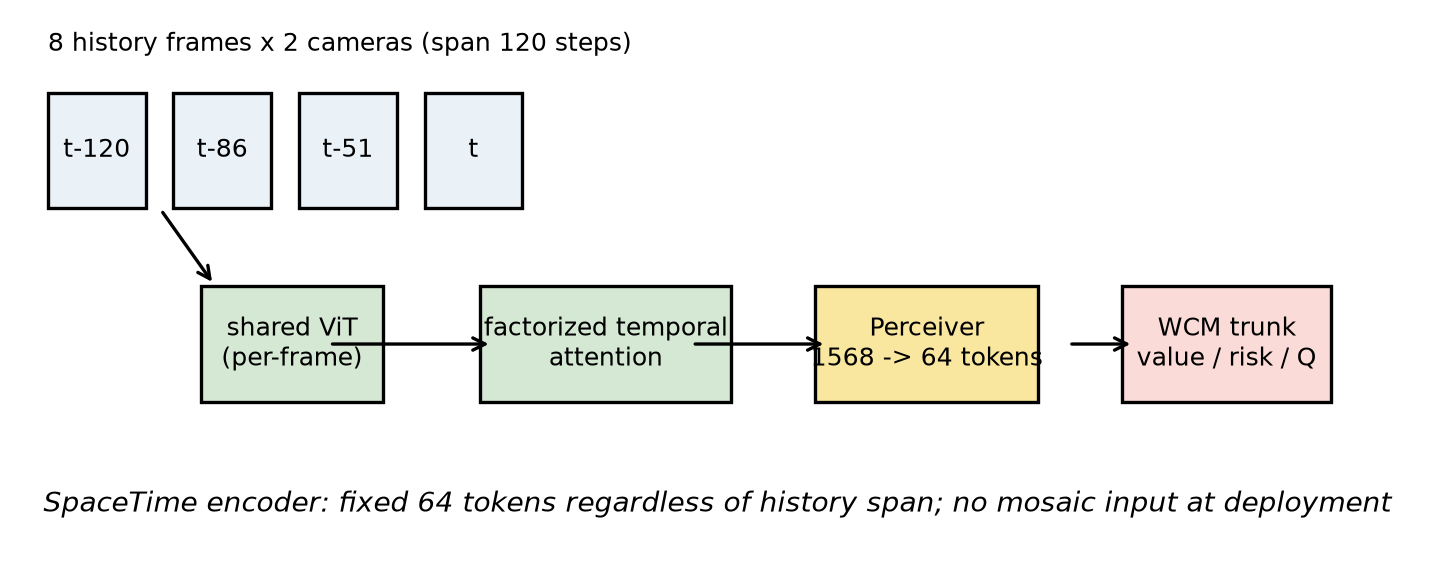
\includegraphics[width=0.88\linewidth]{../assets/figures_wcm_to_spacetime/fig3_architecture.png}
\caption{The fixed-query \SpaceTime{} encoder. Eight sparsely sampled frames are encoded independently, mixed by factorized temporal layers, and compressed to 64 queries before the existing WCM heads.}
\label{fig:architecture}
\end{figure}

\section{Experimental protocol}

\subsection{Models and route}

The main route is
\begin{center}
\fbox{original WCM}\ $\longrightarrow$\ \fbox{T8--$H_{60}$ \SpaceTime{}}\ $\longrightarrow$\ \fbox{T8--$H_{120}$ \SpaceTime{}}.
\end{center}
The four-frame Image-B4 input mosaic is retained as a low-frame reference, not as a point on the same temporal-span axis. It provides a simple history baseline but does not receive the main mechanistic interpretation. A matched eight-frame mosaic experiment is required before making a strong claim that structured \SpaceTime{} encoding is better than input-level frame stacking.

Both \SpaceTime{} spans use the same eight-frame architecture, 64 queries, direct teacher-free deployment, two-stage training (10-epoch joint stage followed by 3-epoch full stage), and initialization from the corresponding same-seed Image-B4 checkpoint. The only model input variable between $H_{60}$ and $H_{120}$ is the offset list.\todo{After seed 1337 is run, replace ``current two-seed'' language where appropriate.}

\subsection{Data and metrics}

The primary evaluation is the 0722 OOD test set. The 0814 5-cut set is a supporting near-distribution evaluation. All paired comparisons use common endpoints and 20,000 episode-level bootstrap resamples. We report MSE as the primary criterion, with Pearson correlation, centered MSE, and mean bias as diagnostics. Efficiency statistics are descriptive and do not enter the performance gate.

\section{Results}

\subsection{Original WCM to T8--$H_{60}$}

On the three-way common OOD endpoint set (125 episodes and 21,832 points), T8--$H_{60}$ improves over the original WCM for both available seeds. The absolute values are shown in Table~\ref{tab:threeway}; the paired intervals against the original WCM are $[-0.12618,-0.11060]$ and $[-0.09314,-0.07849]$ for MSE seeds 3072 and 42, respectively. These results support a system-level improvement claim. They do not isolate the temporal module from differences in training recipe or initialization.

\begin{table}[t]
\centering
\caption{Current three-way OOD results on a common endpoint set. T8--$H_{60}$ denotes the direct \SpaceTime{} model.}
\label{tab:threeway}
\small
\begin{tabular}{llccc}
\toprule
Seed & Metric & Original WCM & Image-B4 mosaic & T8--$H_{60}$ \\
\midrule
3072 & MSE & 0.15167 & 0.04524 & 0.03334 \\
     & Pearson & 0.140 & 0.849 & 0.838 \\
42   & MSE & 0.11036 & 0.05294 & 0.02467 \\
     & Pearson & 0.226 & 0.834 & 0.851 \\
\bottomrule
\end{tabular}
\end{table}

\subsection{Fixed bottleneck, longer span}

Table~\ref{tab:hspan} reports paired comparisons for the post-hoc $H_{120}$ span experiment. The pair endpoints contain 22,082 OOD points; they are not identical to the older three-way endpoint manifest, so absolute MSE values must not be compared across tables as if they were evaluated on exactly the same points. The paired deltas are directly comparable within each pair.

\begin{table}[t]
\centering
\caption{T8--$H_{120}$ paired OOD deltas. Negative $\Delta\mse$ is an improvement.}
\label{tab:hspan}
\small
\begin{tabular}{llcc}
\toprule
Comparison & Seed & $\Delta\mse$ [95\% CI] & $\Delta$ Pearson [95\% CI] \\
\midrule
$H_{120}$ vs Image-B4 & 3072 & $-0.0189$ [$-0.0209,-0.0168$] & $+0.0188$ [$+0.0065,+0.0330$] \\
$H_{120}$ vs Image-B4 & 42 & $-0.0325$ [$-0.0354,-0.0294$] & $+0.0197$ [$+0.0003,+0.0392$] \\
$H_{120}$ vs $H_{60}$ & 3072 & $-0.0069$ [$-0.0089,-0.0050$] & $+0.0297$ [$+0.0184,+0.0434$] \\
$H_{120}$ vs $H_{60}$ & 42 & $-0.0040$ [$-0.0055,-0.0026$] & $+0.0045$ [$-0.0058,+0.0164$] \\
\bottomrule
\end{tabular}
\end{table}

The key controlled comparison is $H_{120}$ versus $H_{60}$: frame count, latent query count, temporal layers, initialization family, and training schedule remain fixed while the maximum offset doubles. Seed 3072 shows a significant Pearson gain; seed 42 shows a positive but non-significant Pearson interval. We therefore describe the span result as consistent for MSE in the current two-seed study, with correlation gains stronger for one seed than the other.

\begin{figure}[t]
\centering
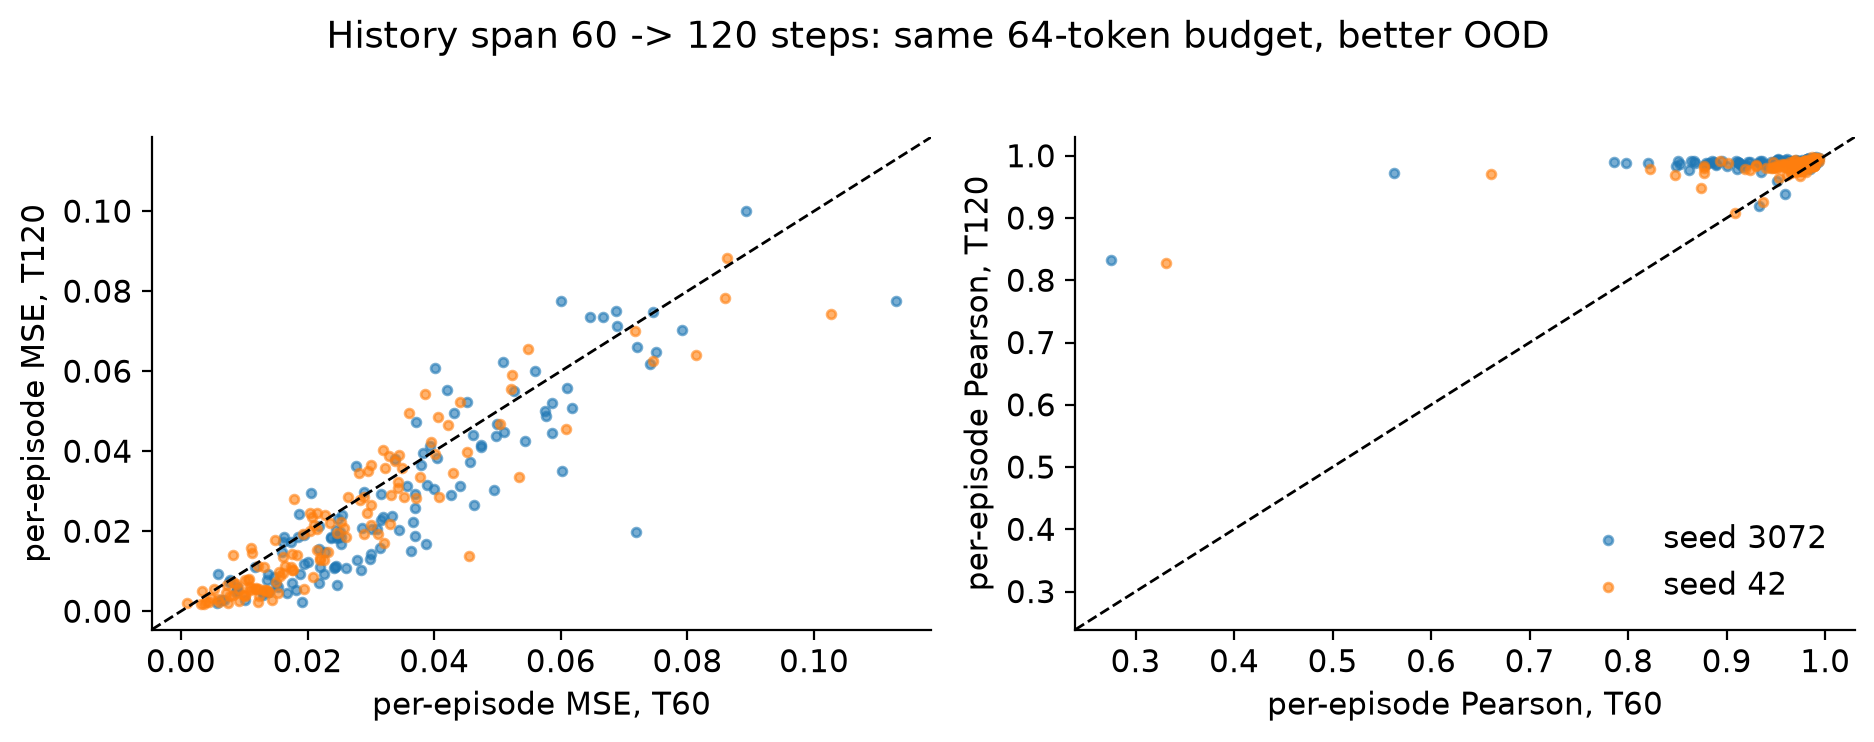
\includegraphics[width=0.92\linewidth]{../assets/figures_wcm_to_spacetime/fig5_span_t60_vs_t120.png}
\caption{Per-episode T8--$H_{60}$ versus T8--$H_{120}$ OOD comparison. The figure uses the pair endpoint manifest and reports the same two seeds as Table~\ref{tab:hspan}.}
\label{fig:span}
\end{figure}

\subsection{Role of the four-frame reference}

The Image-B4 model demonstrates that adding sparse visual context can be useful, but it changes both input organization and the amount of per-frame visual information. The current T8--$H_{60}$ comparison does not pass the pre-registered strong-baseline gate for superiority over this reference because Pearson changes in opposite directions across seeds and the MSE gain is partly explained by bias reduction. We consequently do not claim that \SpaceTime{} is uniformly superior to mosaic.\todo{Add the matched eight-frame mosaic result before making any structured-vs-mosaic claim.}

\optionalfigure{../assets/figures_wcm_to_spacetime/fig6_video_inference.png}{0.96}{Representative video inference with ground-truth return and model predictions. The final caption must state the episode-selection rule and whether the panel was selected before inspecting model outputs.}{fig:video-inference}
\optionalfigure{../assets/figures_wcm_to_spacetime/fig7_analysis.png}{0.96}{Additional diagnostic analysis supplied with the experiment. The caption should identify the measured quantity, split, seed, and whether the visualization is exploratory.}{fig:analysis}

\section{Ablations and analysis}

\subsection{Frame count versus span}

T4/Image-B4 is a low-frame reference. It should not be read as evidence that four, eight, or sixteen frames form a monotone scaling law. The controlled axis in this paper is $H_{60}\rightarrow H_{120}$ at T8 and $K=64$.\todo{Insert the final T4/T8 matched table if the T4 run is retained in the final experiment set.}

\subsection{Efficiency}

The current T8 \SpaceTime{} model has approximately 176.1M parameters, compared with 170.6M for the original WCM and Image-B4 systems. Its measured forward time is about 12.9 ms per sample, versus approximately 6.9 ms for original WCM and 6.1 ms for Image-B4 under the reported batch-four measurement. Thus ``fixed budget'' refers to the latent representation bottleneck, not equal wall-clock cost.

\subsection{What the experiment does not identify}

The reported checkpoints differ in more than one training detail from the original WCM, and current \SpaceTime{} checkpoints are initialized from Image-B4 weights. The results therefore establish a system-level route and controlled span comparison, not a clean causal estimate of every temporal block's marginal contribution. A matched-training three-arm experiment would be needed for that stronger claim.

\section{Limitations and completion criteria}

Two items remain before this draft can be treated as a final empirical paper. First, seed 1337 must be trained and evaluated with the same paired endpoint protocol. Second, an eight-frame input-mosaic control should be added if the paper is to compare structured \SpaceTime{} encoding against mosaic as a mechanism rather than as an engineering reference. Until then, the abstract and conclusion should retain the words ``current two-seed'' and ``provisional''.

The current data also come from one robot task family and one offline value-learning pipeline. The paper does not claim that 64 queries are sufficient for arbitrary histories, that longer spans always help, or that the encoder recovers a causal world model. Those are separate questions for future experiments.

\section{Conclusion}

We presented a bounded route from original WCM to \SpaceTime{}: encode eight visual observations with explicit temporal interaction and compress them into a fixed set of 64 latent queries before value prediction. Holding the frame count and latent bottleneck fixed, extending the sampled span from $H_{60}$ to $H_{120}$ currently lowers OOD MSE in two seeds. The result supports the narrower claim that a fixed latent bottleneck can usefully encode a longer history in this task setting. Completing the third seed and matched eight-frame mosaic control will determine whether that observation is robust enough for a stronger generalization claim.

\bibliographystyle{plainnat}
\bibliography{refs}

\end{document}
